\section{Monte Carlo}

Monte-Carlo methods are a set of randomized algorithms. The general idea is to use random sampling rather than computing to help solve a problem. Such algorithms are mostly used when computing a solution to the problem is not feasible. Because of the use of random sampling, they are heuristical by nature : their results are not always guaranteed to be exact. Throughout the years, Monte-Carlo methods have been successfully used in physics, mathematics  and computer science.\\


In this report, we will be interested in a special case of Monte-Carlo method : Monte-Carlo tree search, aka MCTS. It applies Monte-Carlo principles to tree exploration. The main field of application is artificial intelligence, especially games with very large move space where a complete tree exploration is not possible in reasonable time, such as Chess and Go.

MCTS is composed of four steps : selection, expansion, simulation and backpropagation. Thoses steps are repeated until time runs out, the maximum number of simulated games has been played, a satisfying result is found or whatever condition is relevant. Generally, the more iterations are run, the more accurate is the result.

\begin{figure}
\centering
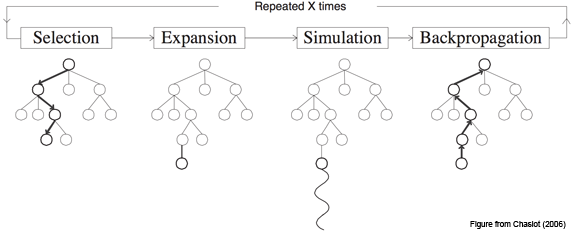
\includegraphics[width=300pt]{mcts-algorithm.png}
\caption{Etapes de Monte-Carlo tree search}
\end{figure}

According to Guillaume Chaslot \cite{ChaPHD} : "MCTS is
applicable if at least the following three conditions are satisfied: (1) the payoffs are bounded
(the game scores are bounded), (2) the rules are known (complete information), and (3) simulations terminate relatively fast (game length is limited)". Those three criterias are verified in the case of the map-coloring game.\\

Dans Monte Carlo, on va chercher à jouer beaucoup de parties pour un graph donné (que nous appellerons le graph étudié) afin de pouvoir jouer les meilleurs coups possibles. 
Pour chaque graph étudié, nous générons un arbre des coups joués où chaque nœuds, sauf la racine, correspondent à des coups joués sur ce graph. 

Ce que contient un nœud de l’arbre généré : 
\begin{itemize}
\item le nœud joué dans le graph étudié
\item la couleur jouée sur ce nœud 
\item le nombre de partie jouées en passant par ce nœud 
\item le nombre de partie gagné par Alice en passant par ce nœud
\end{itemize}

Au début l’arbre ne contient que la racine et les premiers coups possibles. Nous n’avons aucune connaissance des coups qui amènent à colorier proprement le graph étudié ni de ceux qui nous mettrons  dans une situation bloquante. 

Afin de limiter le nombre de fils, nous allons éliminé des coups équivalents : nous considérons que les couleurs sont numérotées et qu’il est impossible de jouer une couleur n, si la couleur n-1 n’a pas encore été jouée. En effet il est équivalent d’introduire la couleur n-1 ou la couleur n. 

D’autre part nous allons généré le graph au fur et a mesure des parties et des coups joués. À chaque fois que l’on est dans un nœud (i.e. on viens de jouer le coup correspondant dans le graph étudié), si il n’a pas de fils, on regarde l'état de la partie : 
\begin{itemize}
\item soit la partie est finie (Alice a gagné ou Bob à gagné), on remonte alors jusqu’à la racine en mettant à jour tous les nœuds sur le chemin. Si Alice a gagné (i.e. le graph étudié est entièrement colorié) on incrémente le nombre de partie joué et le nombre de partie gagné. Si Alice n’a pas gagné (i.e. le graph étudié n’est pas entièrement colorié)  on incrémente juste le nombre de partie joué.
\item soit on peut continuer (auquel cas on génère les fils et on continue la simulation récursivement).
\end{itemize}
Quand on a joué dans un nœud, on a un pourcentage de victoire pour le coup correspondant, mais il n’est pas forcément représentatif. Le fait de jouer plus de parties va permettre de diminuer l'intervalle de confiance de ce ratio de victoire.

\subsection {Algorithme de notre IA}
Pour éviter de toujours passer par les mêmes nœuds, nous allons essayé passer par tous les frères d’un nœud déjà visité avant de pouvoir le revisiter pour explorer ces fils. Ce qui compte, ce sont surtout les coups au premier niveau (le niveau que l’on est en train d’étudier, les coups à jouer immédiatement). Les coups de niveau inférieur ne pourront pas être tous explorés, mais seront regardés de plus près quand on avancera dans le jeu et qu'ils arriveront au premier niveau.
La partie délicate de Monte-Carlo est la sélection de nœud pour l'exploration. Dans un premier temps nous avons considéré  qu’il faut en priorité visiter le nœud qui a le moins de parties jouées, car il a été visité moins de fois que ses « frères ». Mais jouer celui le moins regardé pour l'instant n'est clairement pas la bonne solution sur le long terme. Il faut une solution adaptative, qui va jouer les coups moins regardés au début, puis qui va jouer les meilleurs pour vérifier que ce sont bien les meilleurs. Nous allons donc utiliser les algorithmes de Multi-armed bandit, plus particulièrement UCB1, qui donne de bons résultats.
(ressource en anglais : \url{http://www.chrisstucchio.com/blog/2012/bandit_algorithms_vs_ab.html})
(ressources en français : \url{http://researchers.lille.inria.fr/~munos/master-mva/lecture03.pdf}, \url{http://fr.slideshare.net/cornec/bandits-algo-klucb-par-garivier} )
La seconde partie de Monte Carlo est l'exploitation. Une fois qu'on a effectué assez de simulations, on choisit un nœud pour le jouer "pour de vrai". Là encore, il y a plusieurs solution : on peut en effet prendre le nœud avec le meilleur ratio brut, mais on peut aussi prendre le nœud avec le meilleur ratio au mieux (plus l'intervalle de confiance) ou encore celui avec le meilleur ratio au pire (moins l'intervalle de confiance). 
Sinon, pour la différence entre Alice et Bob, on se base sur une sélection min-max classique. Donc pour Alice on choisit le coup qui a le plus grand nombre de partie gagnée. Et pour Bob on choisit celui qui a le plus petit nombre de partie gagnée. 
